%%%%%%%%%%%%%%%%%%%%%%%%%%
\chapter{Introduction}
\label{chap::intro}
%%%%%%%%%%%%%%%%%%%%%%%%%%

\baselineskip=26pt

\thispagestyle{empty}

\hspace{5mm}With the increasing design
complexity, the amount of buses between different modules on a
chip also increases rapidly. Bus routing has become a major
concern of comparable importance to timing and power in multi-core
SoC designs. To ease the efforts of bus routing in later routing
stage, it is desirable to consider this issue in early floorplanning
stage. Since buses are of different widths and required to go
through different sets of modules, the bus routability
is severely affected by the module position. Bus-driven
floorplanning targets on obtaining a bus-routable floorplan such
that the chip area and the bus area are
minimized. Recently, many bus-driven floorplanning algorithms have
been proposed in the literature \cite {Rafiq02, Xiang03, Chen05,
Law05, Xiang07, Ma08, Kim08_1, Kim08_2, Sheng10, He10, PH10}.
However, these bus-driven floorplanning algorithms
adopt an over-simplified formulation which ignores the practical
issues such as the position and orientation of the bus pin.
Without taking those practical issues into consideration,
it may have the following impacts on bus routing:
\begin{itemize}
\item \textbf{Bus twisting:} It makes the signal wires cross at a
point and decreases accessibilities of the bused pins.
\item \textbf{Via increasing:}
Several vias occur at the bend of a bus that have adverse effects
on the bus delay.
\item \textbf{Delay variation:} Different
driver-load wirelength between different bus bits causes
delay variation among all bus bits.
\end{itemize}

\begin{figure}[htb]
  \centering
    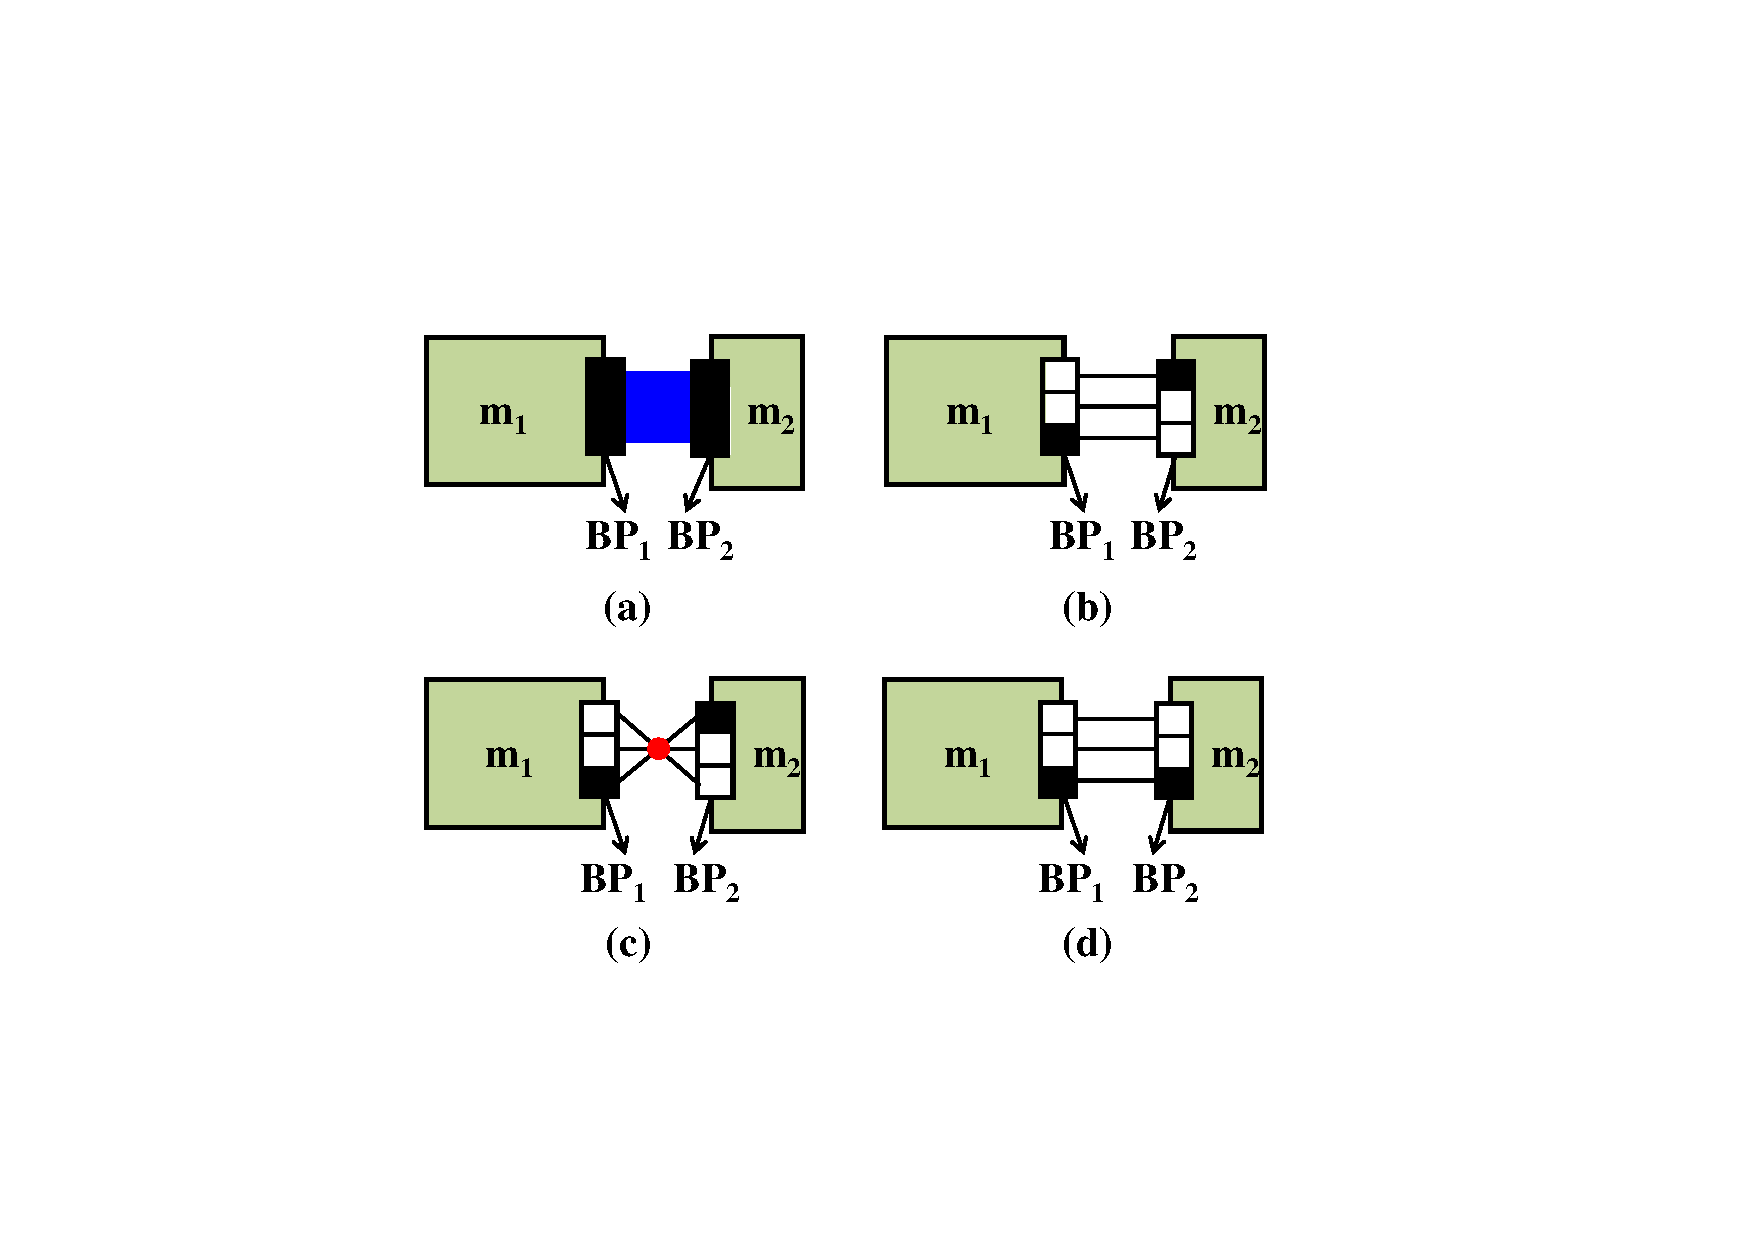
\includegraphics[width=8.8cm]{Fig/bus_twisting.pdf}
    %\centerline{\psfig{figure=Fig/bus_twisting.eps, width=8.8cm}}
     \caption{
      (a) One horizontal bus connects two bus pins. (b) Bus routing without considering the effect of the bus pin. (c) Bus twisting. (d) No bus twisting after flipping the bus pin.
   }
  \label{fig::bus_twisting}
\end{figure}

One example of the bus twisting is given in Figure~\ref{fig::bus_twisting}.
In Figure~\ref{fig::bus_twisting} (a), two modules $m_1$ and $m_2$ are placed
on the floorplan, and two bus pin $BP_1$ and $BP_2$ connected by one horizontal bus
are placed on the boundary of the two modules. Since the effect of the bus pin
is not considered during bus routing in current algorithms,
the routing result in Figure~\ref{fig::bus_twisting} (b)
is obtained, and some bits of the bus pin are not correctly connected
by the wire. Therefore, the wrong signal is transmitted via the bus,
the Most Significant Bit (MSB) of each bus pin is marked with black color
in all figures of this paper.
In this paper, the bus pin is carefully handled during bus routing, thus,
each bus can be correctly connected by the wire as shown in Figure~\ref{fig::bus_twisting} (c).
However, all wires are twisted at one point in the figure,
the problem can be solved by flipping the bus pin $BP_2$ as shown in Figure~\ref{fig::bus_twisting} (d).

Therefore, an over-simplified bus-driven floorplanning formulation will
make the routability and the solution quality in doubt.

\begin{figure}[htb]
  \centering
    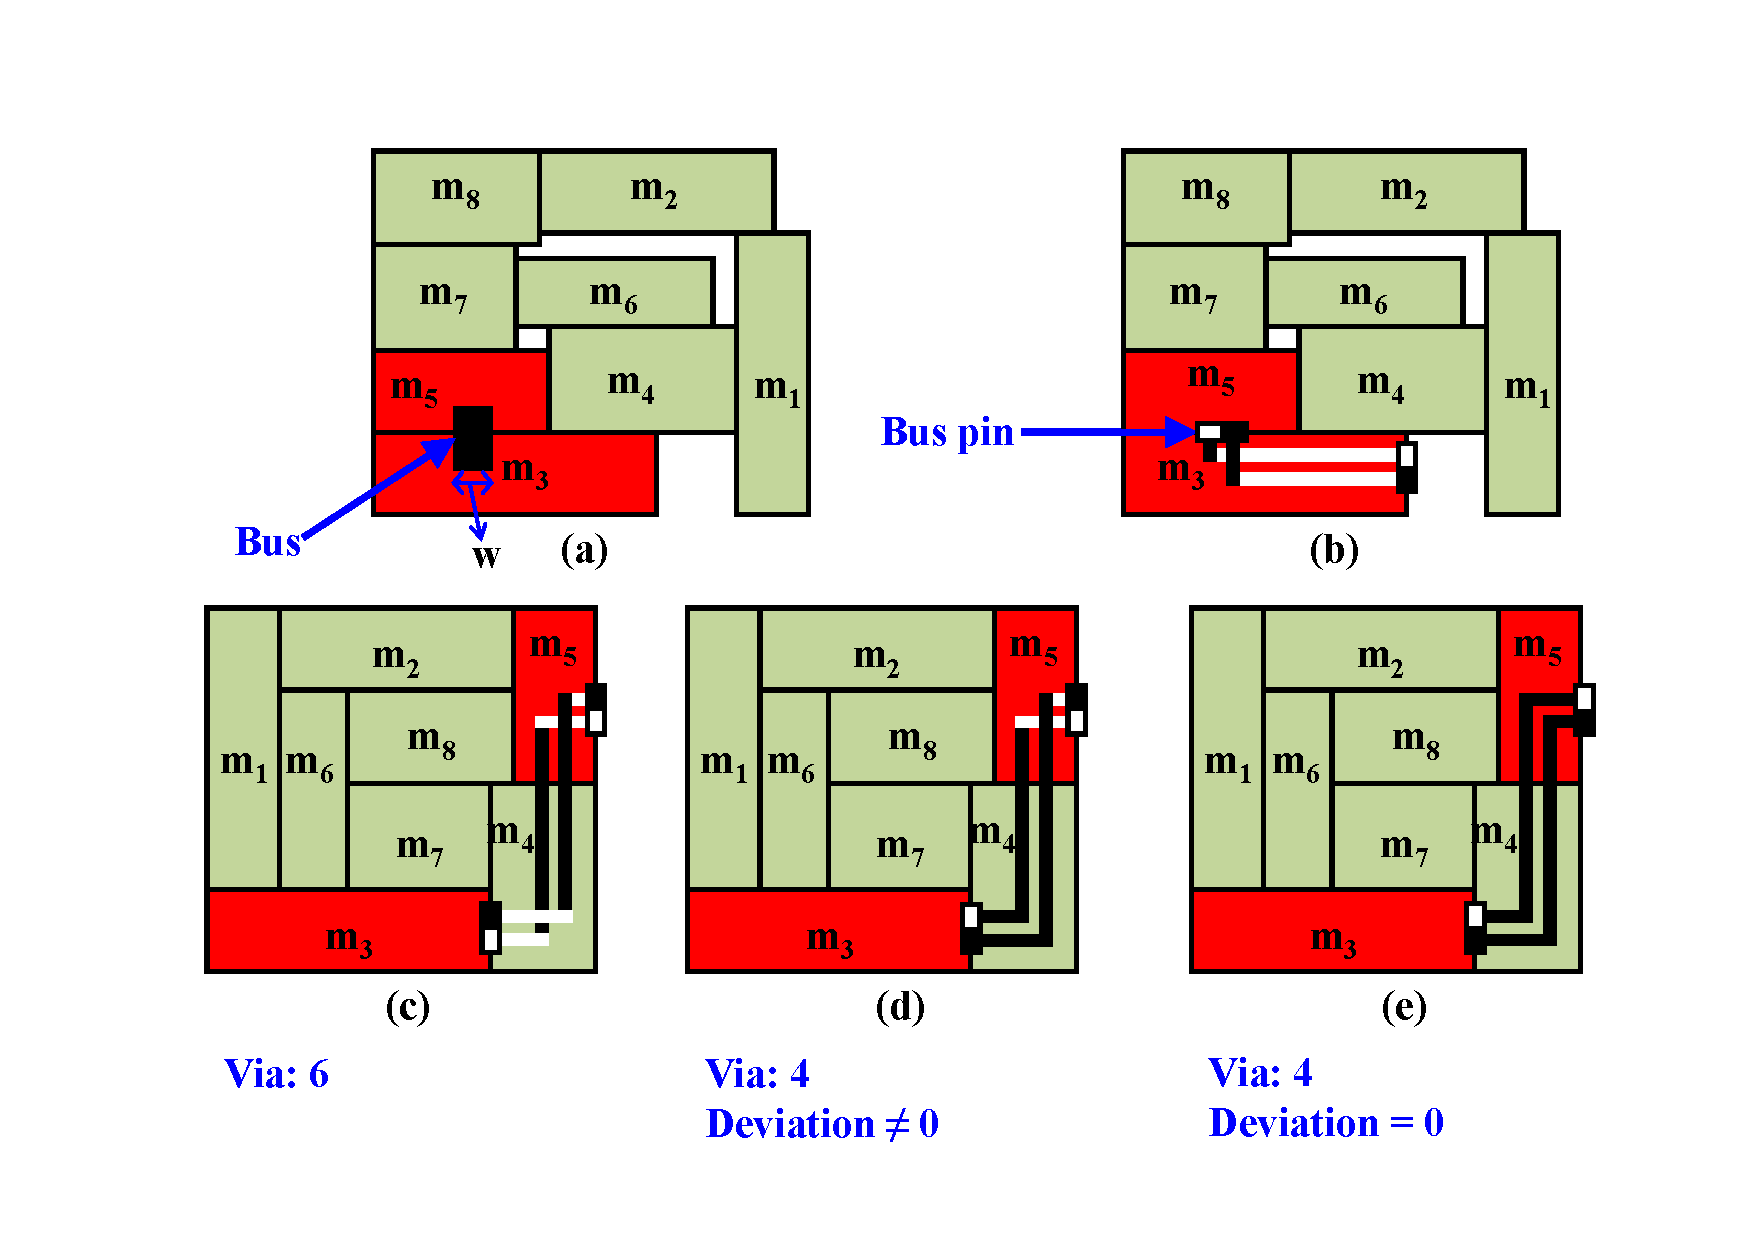
\includegraphics[width=13cm]{Fig/introduction_example.pdf}
    %\centerline{\psfig{figure=Fig/introduction_example.eps, width=13cm}}
     \caption{
      (a) Simplified bus routing. (b) Bus routing considering the bus pin. (c) Bus routing with the diagonal connection between the modules. (d) Via-aware bus routing with the diagonal connection between modules. (e) Bus routing considering both vias and wirelength deviation.
   }
  \label{fig::introduction_example}
\end{figure}

Figure~\ref{fig::introduction_example} illustrates the impact of
the position and orientation of the bus pin. There are eight
modules and one bus that connects two modules $m_3$ and $m_5$,
i.e., bus modules. In Figure~\ref{fig::introduction_example} (a),
existing bus-driven floorplanning algorithms connect $m_3$ and
$m_5$ by simply one vertical bus. However, by considering the
actual positions of the bus pins in
Figure~\ref{fig::introduction_example} (b), the bus pins of these
two modules can not be passed by only one vertical bus, and the
wirelength is much longer than the simplified estimation.

Furthermore, current bus-driven floorplanning algorithms restrict
a bus only bends above the bus modules, i.e., only
horizontal and vertical connections on the bus modules are
allowed. Such restriction limits the flexibility on the bus shape
resulting a narrower solution space. Therefore,
better bus-driven floorplanning solutions may be missed in such
formulation. In this paper, we explore the diagonal connection
between the bus modules to improve the solution quality. Compared with
Figure~\ref{fig::introduction_example} (b), a better solution with
smaller area can be achieved by utilizing the diagonal connection
between $m_3$ and $m_5$ as shown in
Figure~\ref{fig::introduction_example} (c). Although there are two
bends occur at two modules $m_4$ and $m_5$,
no extra vias are required at the bend of $m_5$ since vias exist
anyway to connect to the bus modules $m_5$. Even extra vias are
still required at another bend on the module $m_4$ which is not
a bus module, it can be eliminated by simply flipping the bus
pin on the module $m_3$ and assigning the horizontal and vertical
buses on the module $m_4$ to the same layer as shown in
Figure~\ref{fig::introduction_example} (d).

As mentioned earlier, different driver-load wirelength between bus
bits causes delay variation among all bus bits. At a load,
the wirelength difference among all bus bits is characterized by
\textbf{wirelength deviation}. Different from
Figure~\ref{fig::introduction_example} (d), the driver-load
bus delay among all bus bits is different, the deviation can be
further optimized to 0 by flipping the bus pin on module $m_5$ as
shown in Figure~\ref{fig::introduction_example} (e).

In this paper, we propose a bus-driven
floorplanning algorithm that fully considers the impact of the
bus pins. By fully utilizing the position and orientation of the
bus pins, we can obtain the high-quality results by exploring
flexibility on the bus shape. Moreover, we also
develop two effective algorithms to minimize the wirelength
deviations and two wirelength reduction algorithms to optimize
the total bus wirelength. Experimental results show that our
algorithms are very promising.

\section{Previous Works}
\label{sec::Previous Works}
The bus-driven floorplanning problem has recently attracted a lot of
attention in the literature. Rafiq et al. proposed an integrated
floorplanning for bus-based microprocessor designs \cite{Rafiq02}.
Multiple topologies were produced for each bus, and a mixed
integer/linear programming approach was adopted to arbitrate the
conflicts between different buses. However, the algorithm was limited to
single fanout buses. Xiang et al. \cite{Xiang03}
solved the bus-driven floorplanning problem by using a
sequence pair (SP) representation based on a simulated annealing (SA)
framework. Chen and Chang \cite{Chen05} handled the bus-driven
floorplanning problem based on the B*-tree representation. The
drawback of the above two methods is that all modules are
connected by either horizontal or vertical 0-bend buses; the
solution space is thus restricted when a large number of the modules
are involved for each bus.
The bus shape problem was improved by \cite{Law05}, where
0-bend, 1-bend, and 2-bend buses were allowed. Nevertheless, there are still
limitations on the bus shape. In \cite{Ma08}, a
multi-bend bus-driven floorplanning algorithm was proposed based on
a TCG representation. It has more flexibility on bus shapes and
obtains higher success rate.

In microprocessors and DSPs, many cores are involved and the signals
are transmitted between different cores by the buses which
play an important role in determining the chip performance.
Therefore, some previous works were developed to deal with
such floorplanning in microarchitectural design.
Kim and Lim \cite{Kim08_1} presented a new bus routing algorithm
based on Hanan grids and linear programming. In \cite{Kim08_2},
the authors proposed a bus-aware microarchitectural floorplanning
which addressed the impact of bus routability on performance/power/thermal issues.
However, the above two works aimed on optimizing IPC (Instructions Per Cycle) and
had a different problem formulation from those aforementioned
floorplanners.

There are still many works which consider other constraints during the bus planning.
Xiang et al. \cite{Xiang07} proposed an OPC-friendly bus driven
floorplanning algorithm which carefully designed the pitch
for buses to avoid the forbidden pitch.
Sheng et al. \cite{Sheng10} proposed an approach which was based on a deterministic
algorithm Less Flexibility First, it run in a fixed-outline area and packed hard blocks one after another.
In \cite{He10}, they presented a floorplan revising method which was based on linear
programming model to minimize the number of reducible routing vias with a controllable
loss on the chip area and wirelength.
The authors \cite{PH10} considered the bus pin issue and explored the diagonal connection
which makes the bus shape more flexible and improves the solution quality.

\section{Our Contributions}
\label{sec::Our Contributions}
%bus-driven
In this paper, we propose a bus-driven
floorplanning algorithm that fully considers the impact of the
bus pins. The diagonal connection between
different modules is explored to make the bus shape more flexible which improves
the success rate.
The contributions of this paper are listed as follows:\\
\begin{itemize}
\item \textbf{Deviation Minimization:}
%deviation
We develop two algorithms to
minimize the wirelength deviation for signal integrity of the buses.
First algorithm explores all possible topologies between any two modules,
and it finally concludes some specific bus patterns,
then the best deviation at each module can be quickly obtained from
those specific bus patterns.
In second algorithm, the procedure of determining the deviation at
each module is divided into two steps --- deviation determination and
accumulated deviation update.
During determining the deviation at one module, all the accumulated deviation
from the driver to its neighbors can also be calculated.
Since the procedure of determining the deviation at each module
is divided into two steps, the segment size for each comparison
becomes smaller, then the total bus patterns can be further reduced to 10 types.
Fewer bus patterns stands for less time is needed for searching the possible bus patterns.
Experimental results show that the wirelength deviation can be effectively reduced.

\item \textbf{Diagonal relation:}
%success rate
In this paper, we explore the diagonal relation between different
modules to make the bus shape more flexible, then the modified
graph coloring algorithm is proposed to determine the layer of each
bus. Experimental results show that our algorithm has
1.2$\times$ improvement on the success rate compared with
\cite{Ma08}.

\item \textbf{Wirelength reduction:}
%wirelength reduction
To further enhance the solution quality, we present two wirelength
reduction algorithms to improve the total bus wirelength.
First algorithm reduces the total bus wirelength by minimizing the
overlap between different bus components
(for the multi-bend bus, each horizontal (vertical) part is called a bus component)
during constructing the minimum spanning tree (MST).
The second algorithm is used to optimize the bus wirelength by
adjusting the coordinate of each horizontal (vertical) bus component.
\end{itemize}

The rest of this paper is organized as follows.
Chapter~\ref{chap::PROBLEM FORMULATION} gives the problem
formulation of the bus-driven floorplanning.
%
Chapter~\ref{chap::CONSTRAINTS AND TERMINOLOGIES} defines the
constraints and terminologies used in this paper.
%
Chapter~\ref{chap::ALGORITHM} gives the details of the proposed
bus-driven floorplanning algorithm.
%
Experimental results are shown in
Chapter~\ref{chap::EXPERIMENTAL RESULTS}.
%
Finally, a conclusion will be given in
Chapter~\ref{chap::CONCLUSIONS}.

\vfill\eject

\thispagestyle{empty}
\newpage
